\documentclass[12pt]{article}

%% preamble: Keep it clean; only include those you need
\usepackage{amsmath}
\usepackage[margin = 1in]{geometry}
\usepackage{graphicx}
\usepackage{booktabs}
\usepackage{natbib}

% for space filling
\usepackage{lipsum}
% highlighting hyper links
\usepackage[colorlinks=true, citecolor=blue]{hyperref}


%% meta data

\title{Stats Paper}
\author{Shuiyi Hu\\
  Department of Statistics\\
  University of Connecticut
}

\begin{document}
\maketitle

\begin{abstract}
  In this paper, we propose a pricing model for airbag options 
including discrete monitoring, time-varying barriers, early 
exercise opportunity, and other clauses simultaneously by a 
PDE approach. A closed-form solution is obtained in the classic 
Black-Scholes economy with no early exercise opportunity. For 
the general case, we develop a numerical algorithm and conduct an 
extensive numerical analysis after calibrating the model to 
the CSI 500 index. Greek letters and dynamic hedging are also 
studied.

\end{abstract}


\section{Introduction}
\label{sec:intro}

  Since their seminal papers [\citet{black1973pricing}, \citet{merton1973theory}], option 
pricing theory has been refined and extended in a huge number of 
directions such as jump-diffusion models, stochastic volatility 
models , variance gamma models \citep[e.g.,][]{madan1998variance}, binomial tree models 
and so on.



% roadmap
The rest of the paper is organized as follows.
The data will be presented in Section~\ref{sec:data}.
The methods are described in Section~\ref{sec:meth}.
The results are reported in Section~\ref{sec:resu}.
A discussion concludes in Section~\ref{sec:disc}.


\section{Data}
\label{sec:data}

  Recall linear function.
\begin{equation}
  \label{eq:lm}
  Y \sim X,
\end{equation}

\section{Methods}
\label{sec:meth}

The smallest AIC is 196.47.
\begin{equation}
  \label{eq:slm}
  Rate \sim MaleRatio + X2015 + BlackRate.
\end{equation}

Equation~\eqref{eq:slm} is interesting.

Sometimes I don't want an equation to be numbered such as this one:
\[
  f(x) = \frac{1}{\sqrt{5\pi}} \exp\left( - \frac{x^2}{3} \right),
\]



\section{Results}
\label{sec:resu}

Table~\ref{tab:aic} summarizes results from some models.

\begin{table}[tbp]
  \caption{This is my first table.}
  \label{tab:aic}
\centering
\begin{tabular}{rrr}
  \toprule
model & AIC \\ 
  \midrule
  1 & 205.99 \\ 
  2 & 201.1 \\ 
  3 & 196.47 \\ 
   \bottomrule
\end{tabular}
\end{table}

Figure~\ref{fig:cars} shows the distance against the speed from this dataset.


\begin{figure}[tbp]
  \centering
  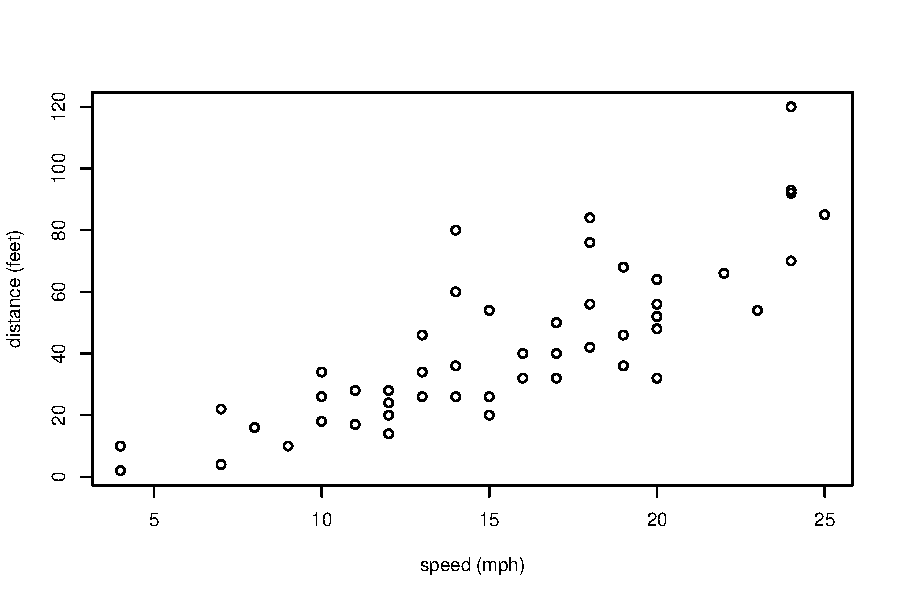
\includegraphics[width=\textwidth]{cars.pdf}
  \caption{This is my first figure.}
  \label{fig:cars}
\end{figure}

\section{Discussion}
\label{sec:disc}

  Structure products are popular in Chinese OTC markets. However, due to 
customer- tailored clauses, it is hard to price them in a unified model. 
In this paper, we study a pricing model for airbag options by incorporating 
discrete monitoring, time-varying barriers, early exercise opportunity and 
other clauses simultaneously based on a PDE approach.

\bibliography{refs}
\bibliographystyle{mcap}

\end{document}